\section{scalability}

Scalability is the ability of a big data system to process
an increasing amount of incoming data by having recourse
to an increasing amount of resources. It can be measured
by the scaleup, the ratio between the amount of data processed
by the model with two different amount of resources but
while being run for the same amount of time.

\begin{figure}[H]
    \begin{center}
        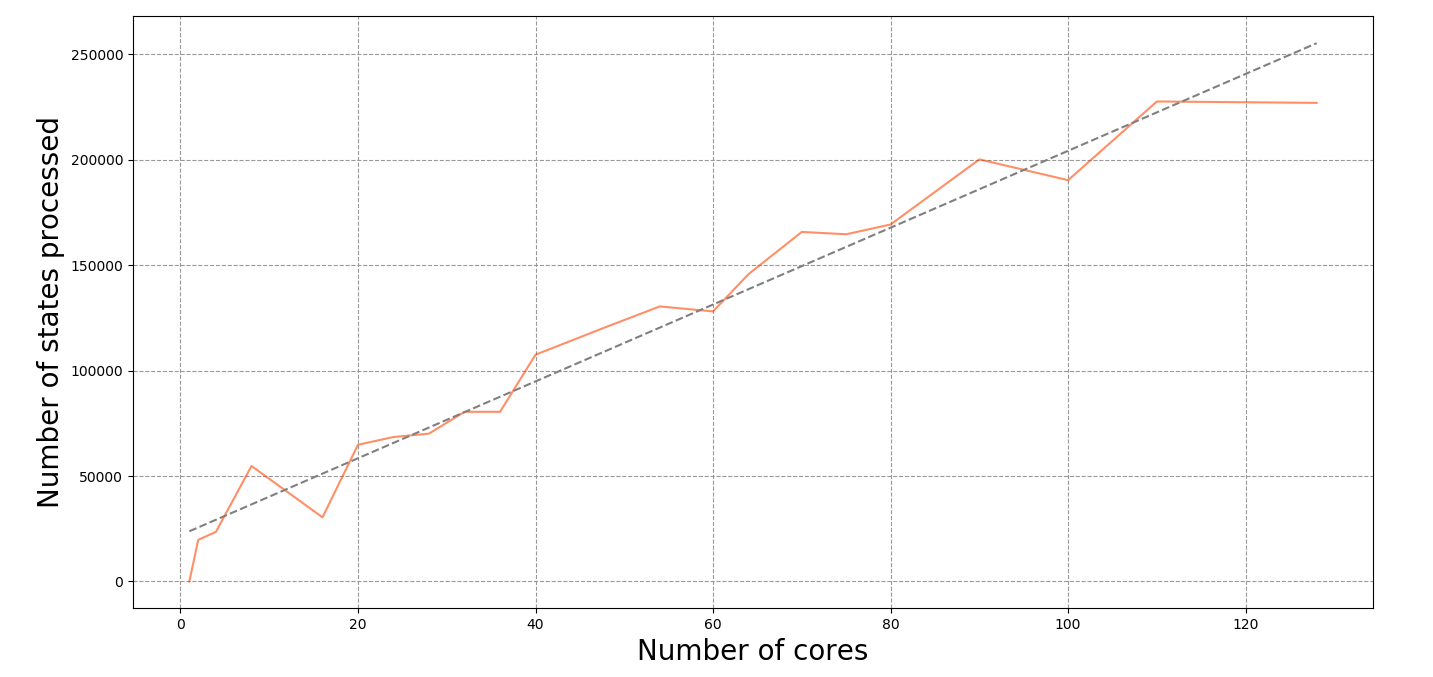
\includegraphics[width=\textwidth, keepaspectratio]{imgs/nmodels.png}
        \caption{Scalability of the RLS algorithm, measured as the number
            of states processed in in a fixed amount of time (timeout of 30 seconds),
            as a function of the number of cores per node in the cluster.}
        \label{nmodels}
    \end{center}
\end{figure}

Scalability is measured as the number of states processed by the last map transformation.
As can be observed in figure \ref{nmodels}, the algorithm's scalability benefits from the addition
of extra cores. Because of the timeout of 30 seconds, much less states are able to reach the last stage
of the pipeline.
